%-----------------------------------------------------------------------------
%
%               Template for sigplanconf LaTeX Class
%
% Name:         sigplanconf-template.tex
%
% Purpose:      A template for sigplanconf.cls, which is a LaTeX 2e class
%               file for SIGPLAN conference proceedings.
%
% Guide:        Refer to "Author's Guide to the ACM SIGPLAN Class,"
%               sigplanconf-guide.pdf
%
% Author:       Paul C. Anagnostopoulos
%               Windfall Software
%               978 371-2316
%               paul@windfall.com
%
% Created:      15 February 2005
%
%-----------------------------------------------------------------------------


\documentclass[10pt]{sigplanconf}

% The following \documentclass options may be useful:

% preprint      Remove this option only once the paper is in final form.
% 10pt          To set in 10-point type instead of 9-point.
% 11pt          To set in 11-point type instead of 9-point.
% authoryear    To obtain author/year citation style instead of numeric.

\usepackage{amssymb}
\usepackage{amsmath}
\usepackage{xcolor}
\usepackage{listings,lstcoq,lsterlang}
\usepackage{bcprules}
%\usepackage{url}
\usepackage{hyperref}
\usepackage{breakurl}
\usepackage{enumitem}

\newtheorem{definition}{Definition}
\newtheorem{theorem}{Theorem}
\newtheorem{lemma}{Lemma}


\lstdefinestyle{default}{
  language=coq,
  basicstyle={\ttfamily\normalsize},
  breaklines=true,
  % frame=tb,
  framesep=6pt,
  captionpos=b,
  numberstyle=\scriptsize,
  numbers=left,
  numbersep=6pt,
  xleftmargin=12pt,
  aboveskip=1em,
  belowskip=1em,
}
\lstdefinestyle{small}{
  style=default,
  basicstyle={\ttfamily\small},
}
\lstset{
  style=default
}

\begin{document}

\special{papersize=8.5in,11in}
\setlength{\pdfpageheight}{\paperheight}
\setlength{\pdfpagewidth}{\paperwidth}

\conferenceinfo{AGERE!@SPLASH}{Oct., 2015, Pittsburgh, PA, USA}
\copyrightyear{20yy}
\copyrightdata{978-1-nnnn-nnnn-n/yy/mm}
\doi{nnnnnnn.nnnnnnn}

% Uncomment one of the following two, if you are not going for the
% traditional copyright transfer agreement.

%\exclusivelicense                % ACM gets exclusive license to publish,
                                  % you retain copyright

%\permissiontopublish             % ACM gets nonexclusive license to publish
                                  % (paid open-access papers,
                                  % short abstracts)

%% \titlebanner{banner above paper title}        % These are ignored unless
%% \preprintfooter{short description of paper}   % 'preprint' option specified.

\title{Actario: A Framework for Reasoning About Actor Systems}
%% \subtitle{Subtitle Text, if any}

\authorinfo{Shohei Yasutake}
           {Tokyo Institute of Technology}
           {yasutake@psg.cs.titech.ac.jp}
\authorinfo{Takuo Watanabe}
           {Tokyo Institute of Technology}
           {takuo@acm.org}

\maketitle

\begin{abstract}
The two main characteristics of the Actor model are asynchronous message passing and dynamic system topology. The latter relies on the on-the-fly creation of actor names that often complicates the formal treatment of systems described in the Actor model. In this paper, we introduce Actario, a formalization of the Actor model in Coq. Actario incorporates a name creation mechanism that is formally proved to generate a consistent set of actor names. The mechanism helps proper handling of names in modeling and reasoning about actor-based systems. Actario also provides a code extraction mechanism that generates Erlang programs.
\end{abstract}

\category{F.3.2}{Logics and Meanings of Programs}%
{Specifying and Verifying and Reasoning about Programs}%
[Mechanical verification]

% general terms are not compulsory anymore,
% you may leave them out
\terms{Actors, Formal Models}

\keywords{Actor Model, Formalization, Actario, Coq, Erlang}

\section{Introduction}
\label{sec:introduction}


The Actor model\cite{Agha:1986aa} is a kind of concurrent computation
model, in which a system is expressed as a collection of autonomous
computing entities called actors that communicate each other only with
asynchronous messages.
On receiving a message, an actor may (1)
send messages to other actors (or itself) whose names are known to the
sender, (2) create new actors and (3) change its behavior for the next
message.

Starting from the 1970s, the Actor model and its variations such as
concurrent objects\cite{Yonezawa:1986aa} have a long research
history. They are today regarded as popular high-level abstractions
for concurrent and parallel programming used in some industrial
strength language and libraries such as Erlang\cite{Erlang},
Scala\cite{Scala} and Akka\cite{Akka}.  Because of this situation,
establishing a mechanized formal verification method for actor-based
systems is a pressing issue.

Several methods and systems for formally verifying actor-based systems
have been presented recently. Rebeca\cite{Sirjani:2011aa} is a
modeling language that allows model-checking.  For deductive
verification using proof assistants, formalizations using
Athena\cite{Musser:2013aa} and Coq\cite{Garnock-Jones:2014aa} have
been presented.

A \emph{name}\footnote{The term \emph{mail address} is used in some other
  literature.} in the Actor model is a unique conceptual location
associated with each actor.  The concept of \emph{name uniqueness}
denotes that each name uniquely refers an actor and each actor should
be referred by a single name.  In the implementations of actor systems
including Erlang, Scala, and Akka, naming of actors is implicit; we
don't need to manually assign a fresh name to a newly created actor.
The name uniquness may be broken if the naming is explicit in complex
systems.  Implicit naming, however, might complicates the formal
treatment of actor-based systems. Thus, some formalization adopts
explicit naming.


In this paper, we propose Actario\cite{Actario}, a Coq framework for
implementing and verifying actor-based systems.  The framework (1)
supports Erlang-like notation for describing an actor system, (2)
allows verifying desired properties of the system using the proof
mechanism in Coq, and (3) generates executable Erlang code from the
system description.

To be close to realistic actor languages and libraries, we designed
Actario to support implicit naming. This is the main difference between
our formalization and formalizations using Athena\cite{Musser:2013aa}
or Coq\cite{Garnock-Jones:2014aa}. The naming mechanism behind the scene
is formally proved to satisfy the name uniqueness.  We also proved other
properties including the persistence of actors and messages.  The proof
scripts of these properties are available in the GitHub repository of
Actario\cite{Actario}.


% 形式的検証をおこなう上での問題
% 特にアクターの名前の生成,一貫性

%% 特にアクターの名前の
%% アクターの名前は必ず一意である必要がある。
%% アクターはシステムの進行に伴って動的に生成されるが、その中で fresh でない名前の生成が行われることはない。
%% fresh なアクターの名前の付け方には、~がある。

% ここで解決したい問題は何か(問題)
% * アクターモデルは並行計算のモデルとして real world でよく使われている
% * 一般的に並行システムの検証は難しい
% * アクターシステム (アクターモデルで記述されたアプリケーション) の検証を行いたい
% Actarioではどのようにして問題を解決しようとしているか(手法)
% 提案手法
% * 名前付けの方法とそれによる名前の一貫性の形式的証明
% それによってどのようなことが明らかになるか:
% * 普通のプログラミングと同様にモデル化できる
% * 名前を勝手につけられるので検証は難しくなる(?)

% Actarioの特徴
% * 普通のプログラミングと同様にシステムを記述できる
% * Coqによって検証もできる
%   + 実装しているシステム自身はCoqによって検証されている
%     - 名前の一貫性(済)
%     - アクターのpersistence (済)
%     - メッセージのpersistence (済)
% * Erlangプログラムを生成できる

The layout of the rest of this paper is as follows.
The next section describes the overview of Actario.
In Section~\ref{sec:semantics}, we give the operational semantics of the Actor model formalized in Actario.
Section~\ref{sec:uniqueness} outlines the proof of the uniqueness property on dynamically generated names.
In Section~\ref{sec:fairness}, we discuss fairness properties formalized in Actario.
The code extraction mechanism is described in Section~\ref{sec:extraction}.
Finally, Section~\ref{sec:relatedwork} overviews related work and Section~\ref{sec:conclusion} concludes the paper.

%% 2節では Actario で使うアクターのシンタックスを説明する。
%% 3節では Actario で用いるアクターモデルの意味論について説明する。
%% 4節では、Actario が用いる意味論において、動的に生成されるアクターの名前が一意になるという定理の証明を説明する。
%% 5節では Actario における fairness の定式化について説明し、
%% 6節で他のアクターモデルの形式化や並行・分散システムの検証用フレームワークとの差異を述べる。

\section{Overview of Actario}
\label{sec:overview}

\subsection{Programming in Actario}

Actario is a Coq framework for defining and verifying actor-based
systems. A typical workflow using Actario is as follows.
\begin{enumerate}
\item Describe an actor system using types and notations defined in the framework.
\item Specify and verify desired properties of the system.
\item Extract the Erlang version of the system using the code extraction mechanism of Coq.
\end{enumerate}
Note that Actario does not provide a dedicated language for describing
actor systems.  The framework offers a set of Coq vocabularies (types
and notations described in Section~\ref{sec:typesandnotations}) for
that purpose.


\paragraph{Example: Recursive Factorial System}
We use a simple example to illustrate a system description in Actario.
Figure~\ref{coq:fact} shows the definition of an actor system that
implements the continuation-passing style factorial function adapted
from \cite{Agha:1986aa}.  In this definition, the function
\lstinline|factorial_system| sets up a system that initially consists
of a single factorial actor whose behavior is defined as
\lstinline|factorial_behv|.  The actor can receive a tuple of a
natural number and the name of a \emph{customer} actor
(\lstinline|cust|) that is intended to receive the result.  If the
first component of tuple is more than zero, \textit{i.e.}, it matches
the successor pattern \lstinline|S n|, the actor creates a new
continuation actor (\lstinline|cont|) and recursively sends itself a
pair of \lstinline|n| and \lstinline|cont|.  The behavior of
continuation actors is specified as \lstinline|factorial_cont_behv|.

\begin{figure}
\begin{lstlisting}[style=small]
Definition factorial_cont_behv (val : nat)
                               (cust : name) :=
  receive (fun msg =>
    match msg with
     | nat_msg arg => cust ! nat_msg (val * arg);
                      become empty_behv
     | _ => become empty_behv
    end).

CoFixpoint factorial_behv :=
  receive (fun msg =>
    match msg with
     | tuple_msg (nat_msg 0) (name_msg cust) =>
       cust ! nat_msg 1;
       become factorial_behv
     | tuple_msg (nat_msg (S n)) (name_msg cust) =>
       cont <- new (factorial_cont_behv (S n) cust);
       me <- self;
       me ! tuple_msg (nat_msg n) (name_msg cont);
       become factorial_behv
     | _ => become factorial_behv
    end).

Definition factorial_system (n : nat) (cust : name) :=
  init "factorial" (
    x <- new factorial_behv;
    x ! tuple_msg (nat_msg n) (name_msg cust);
    become empty_behv
  ).
\end{lstlisting}
\caption{Recursive Factorial System in Actario}\label{coq:fact}
\end{figure}

%% \begin{figure}[t]
%% \centering
%% 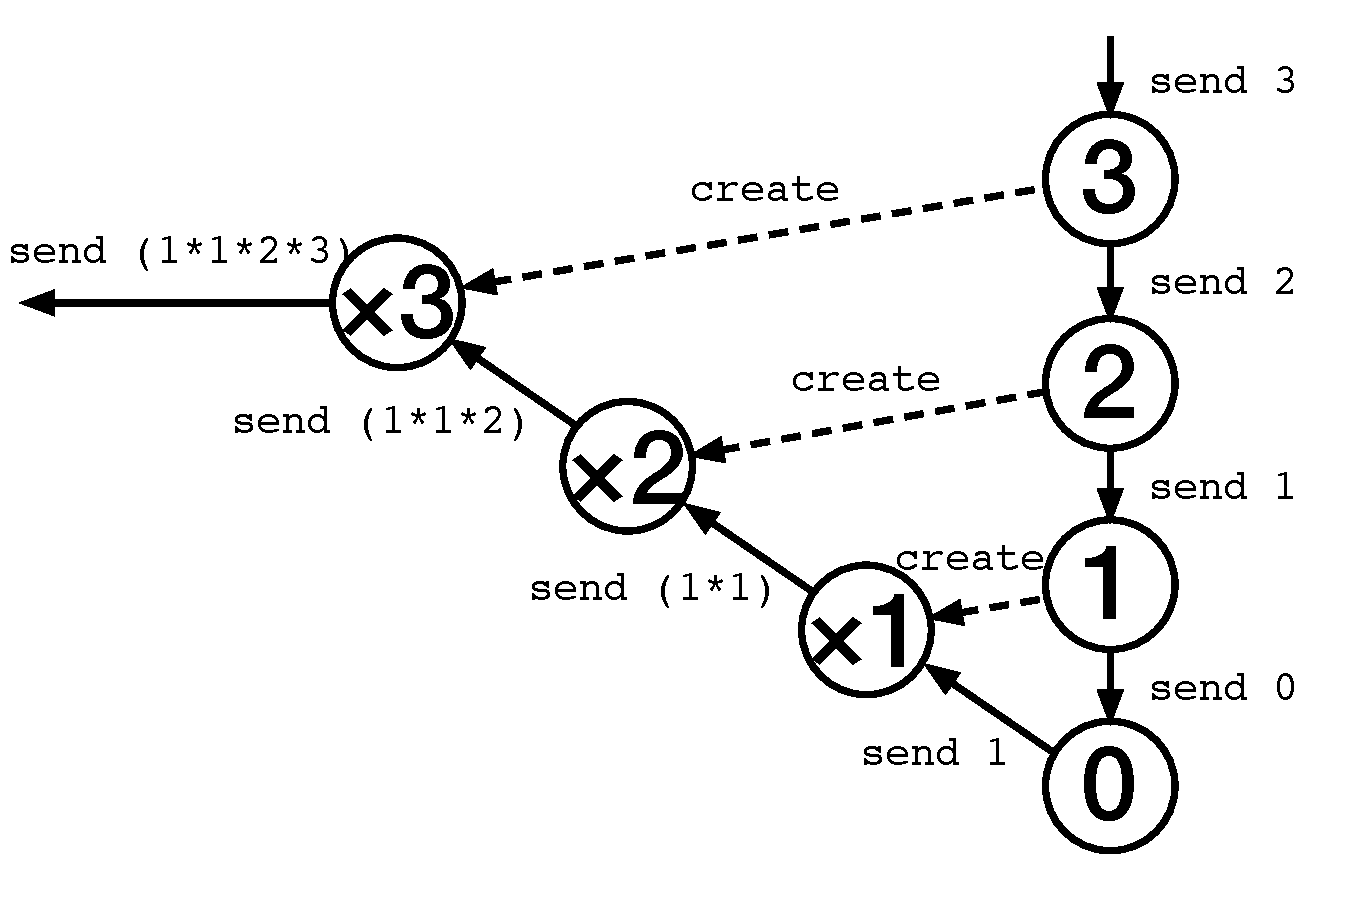
\includegraphics[width=8cm]{./images/fact.pdf}
%% \caption{Recursive Factorial}\label{fig:fact}
%% \end{figure}


\begin{figure}
\begin{lstlisting}
Inductive message : Set :=
 | empty_msg : message
 | name_msg : name -> message
 | str_msg : string -> message
 | nat_msg : nat -> message
 | bool_msg : bool -> message
 | tuple_msg : message -> message -> message.
\end{lstlisting}
\caption{Message Type}\label{coq:message}
%\end{figure}
%\begin{figure}
\hspace*{1em}
\begin{lstlisting}
CoInductive actions : Type :=
 | new : behavior -> (name -> actions) -> actions
 | send : name -> message -> actions -> actions
 | self : (name -> actions) -> actions
 | become : behavior -> actions
with behavior : Type :=
 | receive : (message -> actions) -> behavior.
\end{lstlisting}
\caption{Types for Actions and Behaviors}\label{coq:actions}
\end{figure}

\subsection{Types and Notations}\label{sec:typesandnotations}

\subsubsection{Types}

Figure~\ref{coq:message} shows the inductively defined type of messages delivered
among actors, each of whose constructors corresponds to a kind of
messages.  In the current version of Actario, a message may be empty,
an actor name, a value of basic types (Boolean, natural number or
string), or a tuple of two messages.

Figure~\ref{coq:actions} defines two mutually coinductive types:
\lstinline|actions| and \lstinline|behavior|. They specify sequences
of actions performed by actors and behaviors of actors respectively.
Each constructor of \lstinline|actions| corresponds to a single action embedded in
an action sequence as follows.
\begin{description}

\item[\texttt{new} \(b\) \(f\)] creates a new actor with initial
  behavior \(b\) and applies \(f\) to the name of the created
  actor. Then continues to the action sequence that \(f\) returns.

\item[\texttt{send} \(n\) \(m\) \(\alpha\)] sends message \(m\) to the
  actor with name \(n\) and then continues to action sequence
  \(\alpha\).

\item[\texttt{self} \(f\)] retrieves the name of the actor that executes this
  action and applies \(f\) to it. Then continues to the action sequence
  that \(f\) returns.

\item[\texttt{become} \(b\)] sets \(b\) as the next behavior of the
  actor that executes this action. This action should end an action
  sequence.
\end{description}

In the Actor model, an actor persists indefinitely. Thus, as shown in
Figure~\ref{coq:fact}, that a behavior may have \lstinline|become|
actions that specify itself or other behaviors eventually recurring to
the original one.  The reason for using \lstinline|CoFixpoint| and
defining \lstinline|actions| and \lstinline|behavior| coinductively is
to model such behaviors.


\subsubsection{Notations}

In addition to the types defined above, Actario provides a collection
of notations (syntactic sugaring) described in
Figure~\ref{coq:notation}.  Using the notations, we can write actor
behaviors intuitively without being complicated by CPS.
Figure~\ref{fig:notationexample} compares the descriptions of a simple
action sequence without/with the notations.

\begin{figure}
\begin{lstlisting}
Notation ``n '<-' 'new' behv ; cont'' :=
    (new behv (fun n => cont))
    (at level 0, cont at level 10).
Notation ``n '!' m ';' a'' :=
    (send n m a) (at level 0, a at level 10).
Notation ``me '<-' 'self' ';' cont'' :=
    (self (fun me => cont))
    (at level 0, cont at level 10).
\end{lstlisting}
\caption{Notations for Actions}\label{coq:notation}
\end{figure}

\begin{figure}\centering
\begin{minipage}{0.2\textwidth}\centering
\begin{lstlisting}[frame=single]
new $b$ (fun x =>
self (fun s =>
send x (name_msg s)
(become $b'$)))
\end{lstlisting}
(a) without notations
\end{minipage}
\hspace*{3ex}
\begin{minipage}{0.2\textwidth}\centering
\begin{lstlisting}[frame=single]
x <- new $b$;
s <- self;
x ! (name_msg s);
become $b'$
\end{lstlisting}
(b) with notations
\end{minipage}
\caption{Example Use of Notations}\label{fig:notationexample}
\end{figure}

\section{semantics}
\label{sec:semantics}

In this section, we explain the formalization of operational semantics of the Actor model in Actario.
First, for the explanation of formalization of operational semantics, we describe \lstinline|name| type, \lstinline|actor| type, \lstinline|in_flight_message| type, and \lstinline|config| type.
And then, we explain how to formalize the operational semantics in Actario.

\subsection{Actor Name}
In Actario, actor name is defined as disjoint sum of the actor with no parent and the actor generated by another actor (Figure \ref{coq:name}).
We call the actor with no parent \textit{toplevel actor}.
This represents initial actors in the system.
And we call the actor generated by another actor \textit{generated actor}.
The name of a generated actor consists of the name of parent actor and the number that the parent actor generated so far.
We call the number \textit{generation number}.
To keep name uniqueness, we introduce generation number.
For more detail about name uniqueness, see section \ref{sec:uniqueness}.

%% Actario ではアクターの名前は、親がいないアクターと何らかのアクターから生成されたアクターに分けて定義する (図\ref{coq:name})。
%% 親がいないアクターは toplevel actor と呼ぶ。
%% これはアクターシステムに最初から存在するアクターを表す。
%% 何らかのアクターから生成されたアクターを generated actor と呼ぶ。
%% generated actor の名前は、親アクターの名前と、その親アクターが何番目に生成した子かという番号 (generation number) のペアとする。
%% これは動的に生成されうるアクターの名前の一意性を保つためである。

\begin{figure}[t]
  \begin{lstlisting}
    Inductive name : Set :=
    | toplevel : string -> name
    | generated : nat -> name -> name.
  \end{lstlisting}
  \caption{name}\label{coq:name}
\end{figure}


\subsection{actor}
We explain how \lstinline|actor| is defined in Actario.
Actor consists of its name, sequence of remaining actions, and next generation number to use in generating next child (Figure \ref{coq:actor}).
If remaining actions are only \textsf{become}, the actor is ready for receiving a message.
%% アクターは、自分自身名前、残りのアクションの列、次回アクターを生成する際に使う generation number の3つのレコード型である (図\ref{coq:actor})。
%% 残りのアクションの列が become のみの場合、このアクターはメッセージを受け取れる状態にあるということを表す。

\begin{figure}[t]
  \begin{lstlisting}
    Record actor := {
      actor_name : name;
      remaining_actions : actions;
      next_num : gen_number
    }.
  \end{lstlisting}
  \caption{actor}\label{coq:actor}
\end{figure}

\subsection{in flight message}
Next, we define \lstinline|in_flight_message| type which represents messages in flight in the configuration.
\lstinline|in_flight_message| consists of the name of destination, the name of sender, and the content of the message (Figure \ref{coq:inflight}).

宛先と送り主とメッセージの内容からなるレコード型である (図\ref{coq:inflight}))。
まだ受け取られていないメッセージを表す。
configuration に用いる。

\begin{figure}[t]
  \begin{lstlisting}
    Record in_flight_message := {
      to : name;
      from : name;
      content : message
    }.
  \end{lstlisting}
  \caption{in flight message}\label{coq:inflight}
\end{figure}

\subsection{configuration}
\textit{configuration} represents snapshot of the actor system.
configuration is used to formulate operational semantics of the Actor model.
In Actario, configuration consists of a list of actors and a list of messages in flight.

\begin{figure}[t]
  \begin{lstlisting}
    Record config := {
      in_flight_messages : list in_flight_message;
      actors : list actor
    }.
  \end{lstlisting}
  \caption{config}\label{coq:config}
\end{figure}


\subsection{label}
Actario formulates operational semantics of the Actor model as labeled transition system, so we define label (Figure \ref{coq:label}).
The explanations of each label are as follows.

%% Actario ではアクターモデルの操作的意味を labeled transition system として定式化するため、ラベルを定義する (図\ref{coq:label}))。
%% 以下にそれぞれの説明を示す。

\begin{description}[style=nextline,leftmargin=12pt,parsep=0pt]
\item[\texttt{Receive (to : name) (from : name) (content : message)}]
  This represents that the actor named \lstinline|to| receives the message \lstinline|content| sent from the actor named \lstinline|from|.
  %% \texttt{to} という名前のアクターが \texttt{from} という名前のアクターからのメッセージ \texttt{content} を受け取って遷移したということを表す。
\item[\texttt{Send (from : name) (to : name) (content : message)}]
  This represents that the actor named \lstinline|from| sends the message \lstinline|content| to the actor named \lstinline|to|.
  %% \texttt{from} という名前のアクターが \texttt{to} という名前のアクターに向けてメッセージ \texttt{content} を送ってシステムが遷移したということを表す。
\item[\texttt{New (child : name)}]
  This represents that the actor named \lstinline|child| is generated.
  %% \texttt{child} という名前の新しいアクターが生成されてシステムが遷移したということを表す。
\item[\texttt{Self (me : name)}]
  This represents that the actor named \lstinline|me| gets the name itself.
  %% \texttt{me} という名前のアクターが自分自身の名前を読みだしたということを表す。
\end{description}


\begin{figure}[t]
  \begin{lstlisting}
Inductive label :=
| Receive (to : name) (from : name) (content : message)
| Send (from : name) (to : name) (content : message)
| New (child : name)
| Self (me : name).
  \end{lstlisting}
  \caption{label}\label{coq:label}
\end{figure}


\subsection{semantics}

We formulate operational semantics of the Actor model as labeled transition system.
For later explanation, we define the symbols as shown in the figure \ref{fig:config}.
%% アクターモデルの操作的意味を configuration のラベル付き遷移システムとして定式化する。
%% これ以降用いる記号を図\ref{fig:config}のように定義する。

\begin{figure}[t]
  \begin{displaymath}
    \begin{array}{rclcl}
      c & \in & \textit{Configuration} & =   & \textit{Set(InFlight)} \times \textit{Set(Actor)} \\
      a & \in & \textit{Actor}  & =   & \textit{Name} \times \textit{Actions} \times \mathbb{N} \\
      n & \in & \textit{Name}   & ::= & \textsf{toplevel}(s) \mid \textsf{generated}(g, n) \\
      m & \in & \textit{Message} & =  & \textit{Name} + \textit{PrimVal} + \\
        &     &                 &     & \textit{Message} \times \cdots \times \textit{Message} \\
      i & \in & \textit{InFlight} & = & \textit{Name} \times \textit{Name} \times \textit{Message} \\
      b & \in & \textit{Behavior} & = & \textit{Message} \rightarrow \textit{Actions} \\
      \alpha & \in & \textit{Actions} & ::= & \textsf{send}(n, m, \alpha) \\
        &     &                 &   | & \textsf{new}(b, \kappa) \\
        &     &                 &   | & \textsf{self}(\kappa) \\
        &     &                 &   | & \textsf{become}(b) \\
      l & \in & \textit{Label}  & ::= & \textsf{Receive}(n, n, m) \\
        &     &                 &   | & \textsf{Send}(n, n, m) \\
        &     &                 &   | & \textsf{New}(n) \\
        &     &                 &   | & \textsf{Self}(n) \\
      \kappa & \in & \textit{Name} \rightarrow \textit{Actions} & & \\
      g & \in & \mathbb{N} & &
    \end{array}
  \end{displaymath}
  \caption{Configuration}\label{fig:config}
\end{figure}

The labeled transition system used in Actario is defined like figure \ref{fig:semantics}.
The explanations for each of transitions are the followings.
%% このラベル一つ一つに対応した意味論は図\ref{semantics}にある。
%% receive はメッセージ待ち状態にあるアクターが、自身に向けて送られたメッセージを受け取り、アクションの列を生成する遷移である。

\begin{description}[style=nextline,leftmargin=12pt,parsep=0pt]
\item[\textsc{Receive}]
  \textsc{Receive} is the transition for \textsf{Receive} label.
  The actor which is ready to receive a message, in other words, the actor whose remaining actions are only \textsf{become}, receives a message and generate new remaining actions by the behavior and the content of the message.
\item[\textsc{Send}]
  \textsc{Send} is the transition for \textsf{Send} label.
  The actor which want to send a message sends a message, and then the message is added into messages in flight.
\item[\textsc{New}]
  \textsc{New} is the transition for \textsf{New} label.
  An actor generates its child actor by the given behavior.
  And then, do the followings:
  \begin{itemize}
  \item The child actor is added into the configuration. The next generation number of child actor is 0.
  \item The next generation number of the parent actor increase by 1.
  \item The child actor is ready to receive a message.
  \end{itemize}
\item[\textsc{Self}]
  \textsc{Self} is the transition for \textsf{Self} label.
  An actor gets the self name and applies it to the continuation.
\end{description}

The definition in Actario is in Appendix \ref{app:lts}.

\begin{figure*}[t]
  \begin{displaymath}
    \begin{array}{rcll}
      (I \uplus \{(n_{\textrm{to}}, n_{\textrm{from}}, m)\}, A \cup \{(n_{\textrm{to}}, \textsf{become}(b), g)\}) &
      \overset{\textsf{Receive}(n_{\textrm{to}}, n_{\textrm{from}}, m)}{\leadsto} &
      (I, A \cup \{(n_{\textrm{to}}, b(m), g)\}) &
      \textsc{(Receive)} \\[1ex]

      (I, A \cup \{(n_{\textrm{from}}, \textsf{send}(n_{\textrm{to}}, m, \alpha), g)\}) &
      \overset{\textsf{Send}(n_{\textrm{from}}, n_{\textrm{to}}, m)}{\leadsto} &
      (I \uplus \{(n_{\textrm{to}}, n_{\textrm{from}}, m)\}, A \cup \{(n_{\textrm{from}}, \alpha, g)\}) &
      \textsc{(Send)} \\[1ex]

      (I, A \cup \{(n, \textsf{new}(b, \kappa), g)\}) &
      \overset{\textsf{New}(n')}{\leadsto} &
      (I, A \cup \{(n, \kappa(n'), g + 1), (n', \textsf{become}(b), 0)\}) & \\
      & & \hfill \textrm{where}\ n' := \textsf{generated}(g, n) &
      \textsc{(New)} \\[1ex]

      (I, A \cup \{(n, \textsf{self}(\kappa), g)\}) &
      \overset{\textsf{Self}(n)}{\leadsto} &
      (I, A \cup \{n, \kappa(n), g\}) &
      \textsc{(Self)}
    \end{array}
  \end{displaymath}
  \caption{labeled transition semantics}\label{fig:semantics}
\end{figure*}

\section{Name Uniqueness}
\label{sec:uniqueness}
%% \note{なぜこれが証明されていなければいけないのか、これが証明されていることによってどういうことが言えるのか}
In programming languages or libraries providing the Actor model such as Erlang or Akka,
the system automatically generates actors with fresh names without specifying the name explicitly by the programmer.
In Actario, the proposition that all actor names in the configuration are not duplicate by any transitions is proven.

%% アクターモデルを提供する言語やライブラリ、例えば Erlang や Akka では、アクターを生成する際にプログラマが名前を指定せずとも fresh な名前を生成してくれる。
%% また、アクターはシステムの進行中に動的に生成されうるものなので、動的に生成されうるアクターの名前が常に一意になることが重要である。
%% Actario では、Actario の意味論において、ある制限を満たした初期状態からの任意の遷移でアクターの名前が衝突しないことを証明した。

To prove, we define an invariant about actor names preserved between any transitions. It is named \textit{trans invariant}.
The trans invariant consists of the following three predicates for configuration.
%% システムの遷移において満たされる、名前についての性質 trans invariant を定義し、trans invariant が確かに遷移の間で保存されることを証明、そして trans invariant が成り立てば名前の一意性が成り立つことの証明、初期状態が

\begin{displaymath}
  \begin{array}{l}
    \texttt{trans\_invariant}(c) := \\
    \quad \texttt{chain}(c) \wedge \texttt{gen\_fresh}(c) \wedge \texttt{no\_dup}(c)
  \end{array}
\end{displaymath}

The brief explanations of \texttt{chain}, \texttt{gen\_fresh}, and \texttt{no\_dup} are followings:

\begin{description}[style=nextline,leftmargin=12pt,parsep=0pt]
\item[\texttt{chain}]
  For each actor in the configuration, if the actor is generated by another actor, then the parent actor is also in the configuration.
\item[\texttt{gen\_fresh}]
  For each actor in the configuration, actor name genereted by the actor in the next is fresh.
\item[\texttt{no\_dup}]
  For all actor name in the configuration are unique.
\end{description}

\subsection{functions}

Before starting the explanation and the proof, we define some functions used in this section.

\begin{description}[style=nextline,leftmargin=12pt,parsep=0pt]
\item[\texttt{actors} $: \textit{Configuration} \rightarrow \textit{Set(Actor)}$]
  \texttt{actors} returns the set of actors in the given configuration.
\item[\texttt{parent} $: \textit{Actor} \rightarrow \textit{Actor}$]
  \texttt{parent} returns the parent actor of the given actor.
  If the given actor is toplevel actor, the function returns nothing. % null?
\item[\texttt{gen\_number} $: \textit{Actor} \rightarrow \mathbb{N}$]
  \texttt{gen\_number} returns generated number of the name of the given actor.
  If the given actor is toplevel actor, the function returns nothing.
\item[\texttt{next\_number} $: \textit{Actor} \rightarrow \mathbb{N}$]
  \texttt{next\_number} returns next generation number of the given actor.
\item[\texttt{name} $: \textit{Actor} \rightarrow \textit{Name}$]
  \texttt{name} returns the name of the given actor.
\item[\texttt{names} $: \textit{Set(Actor)} \rightarrow \textit{Set(Name)}$]
  \texttt{names} returns names of the given set of actors.
\end{description}

\subsection{chain}
We define an predicate of configuration, called \texttt{chain}.
\texttt{chain} is the predicate that, for each actor in the given configuration, if it is generated by another actor, the parent actor is also in the configuration.
\texttt{chain} is defined as the following.

\begin{displaymath}
  \begin{array}{l}
    \texttt{chain}(c) := \\
    \quad \forall a \in \texttt{actors}(c), \exists p, p = \texttt{parent}(a) \Rightarrow p \in \texttt{actors}(c)
  \end{array}
\end{displaymath}

Then, we can prove \textit{chain preservation property} that chain is preserved between any transitions.
The proof is by case analysis on the label.
\texttt{chain} is decided by only actor names, and the transition which have a possibility to change the names in the configuration is only \textsc{New} transition.
Therefore, we consider only the case of \textsc{New} transition.

\begin{lemma}{chain preservation}
\begin{displaymath}
  \begin{array}{l}
    \forall c, c' \in \textit{Configuration}, \forall l \in \textit{Label}, \\
    \quad \texttt{chain}(c) \wedge c \overset{l}{\leadsto} c' \Rightarrow \texttt{chain}(c')
  \end{array}
\end{displaymath}
\end{lemma}

\subsection{gen\_fresh}
We define \texttt{gen\_fresh} predicate that, for each actor in the configuration, the name of its child is always fresh.
The definition of \texttt{gen\_fresh} is complicated a little.
We translate the proposition that next generated name is fresh to the following.

\begin{displaymath}
  \begin{array}{l}
    \texttt{gen\_fresh}(c) := \\
    \quad \forall a \in \texttt{actors}(c), \exists p, p = \texttt{parent}(a) \wedge \quad \quad p \in \texttt{actors}(c) \Rightarrow \\
    \texttt{gen\_number}(a) < \texttt{next\_number}(p)
  \end{array}
\end{displaymath}


It is guaranteed that the actor name generated in the next is fresh if satisfying \texttt{gen\_fresh} predicate by the relation of next generation numbers and actor names. %% For each actor in the configuration, if its parent is in the configuration, the next generation number of the parent actor is greater than the generation number of the name of the child actor.
However, the actor name generated after the next is not always fresh name.
For example, if there are two actors ($A$ and $B$) that have the same name and the same next generation number and actor $A$ generates a child actor and actor $B$ generates a child actor, although \texttt{gen\_fresh} holds, these child actors have the same name.
Furthermore, if the parent of the actor $A$ does not exist in the configuration and the parent of the parent exists in the configuration, and the parent of the parent actor generates an actor and it also generates an actor, then the name is possible to have the same as $A$'s one.

%% つまり、あるアクターについて、システム内に親アクターがいる場合、親アクターが次に生成する番号は自分の番号よりも大きい、ということにより、次に生成するアクターの名前が被らないようになっている。
%% ただし、次に生成するアクターの名前は fresh でもその次に生成するアクターは fresh ではないこともある。
%% 例えば、同じ名前でかつ次の generation number も同じという2つのアクターがいた場合、まず片方のアクターが生成するアクターの名前は fresh だが、その次にもう片方のアクターがアクターを生成したとすると、名前が被ってしまう。
%% また、親アクターがシステム内に存在せずに、親の親は存在しているという場合、親の親が次に生成するアクターの名前は被らないが、その子アクターが次に生成する名前は被ってしまう可能性がある。(図?)

Thus, to prove \textit{gen fresh preservation} proposition that \texttt{gen\_fresh} is preserved between transitions, it is necessary to use \texttt{chain} and \texttt{no\_dup} as hypotheses.
%% The proof is by ...
%% 以上のように gen\_fresh だけでは gen\_fresh を導けないので、gen\_fresh の証明には chain と no\_dup の性質が必要になる。

\begin{lemma}{gen fresh preservation}
\begin{displaymath}
  \begin{array}{l}
    \forall c, c' \in \textit{Configuration}, \forall l \in \textit{Label}, \\
    \quad \texttt{chain}(c) \wedge \texttt{gen\_fresh}(c) \wedge \texttt{no\_dup}(c) \wedge c \overset{l}{\leadsto} c' \Rightarrow \\
    \quad \texttt{gen\_fresh}(c')
  \end{array}
\end{displaymath}
\end{lemma}

\subsection{no\_dup}
We define \texttt{no\_dup} predicate that all actor names in the given configuration are unique.
This is the property we have to prove.
\texttt{no\_dup} is defined as the following.

\begin{displaymath}
  \begin{array}{l}
    \texttt{no\_dup}(c) := \\
    \quad \forall a \in \texttt{actors}(c), \texttt{name}(a) \notin
    \texttt{names}(\texttt{actors}(c) \setminus \{a\})
  \end{array}
\end{displaymath}

We proved \textit{no dup preservation} property defined as the following.
It represents that if the actor names in the configuration is not duplicate and the next generated actor name is fresh, then \texttt{no\_dup} holds in the next configuration.

\begin{lemma}{no dup preservation}
\begin{displaymath}
  \begin{array}{l}
    \forall c, c' \in \textit{Configuration}, \forall l \in \textit{Label}, \\
    \quad \texttt{gen\_fresh}(c) \wedge \texttt{no\_dup}(c) \wedge c \overset{l}{\leadsto} c' \Rightarrow \texttt{no\_dup}(c')
  \end{array}
\end{displaymath}
\end{lemma}

\subsection{uniqueness}
Then, we start to prove name uniqueness.
First, we prove trans invariant preservation that trans invariant is preserved between transitions.
This is obvious by chain preservation, gen fresh preservation and no dup preservation.
\begin{lemma}{trans invariant preservation}
  \begin{displaymath}
    \begin{array}{l}
      \forall c, c' \in \textit{Configuration}, \forall l \in \textit{Label}, \\
      \quad \texttt{trans\_invariant}(c) \wedge c \overset{l}{\leadsto} c' \Rightarrow \texttt{trans\_invariant}(c')
    \end{array}
  \end{displaymath}
\end{lemma}

Next, we prove that if trans invariant holds in initial configuration, trans invariant holds after arbitrary transitions.

%% 次に初期状態について trans\_invariant が成り立っていれば、任意回の遷移後も trans\_invariant が成り立つということをを証明する。

\begin{lemma}{trans invariant preservation star}
  \begin{displaymath}
    \begin{array}{l}
      \forall c, c' \in \textit{Configuration}, \forall l \in \textit{Label}, \\
      \quad \texttt{trans\_invariant}(c) \wedge c \overset{l}{\leadsto\star} c' \Rightarrow \texttt{trans\_invariant}(c')
    \end{array}
  \end{displaymath}
\end{lemma}
$c \overset{l}{\leadsto\star} c'$ represents reflexive transitive closure of transition.
The proof is by induction of reflexive transitive closure of transition and trans invariant preservation.

Finally, we can prove name uniqueness.
\begin{theorem}{name uniqueness}
  \begin{displaymath}
    \begin{array}{l}
      \forall c, c' \in \textit{Configuration}, \forall l \in \textit{Label}, \\
      \quad \texttt{trans\_invariant}(c) \wedge c \overset{l}{\leadsto\star} c' \Rightarrow \texttt{no\_dup}(c')
    \end{array}
  \end{displaymath}
\end{theorem}
This is obvious by trans invariant preservation star because \texttt{no\_dup} is in \texttt{trans\_invariant}.

\section{Fairness}

\textsf{fairness} is a property that reception of a message does not delay infinitely.
There are two variants of fairness property, weak fairness and strong fairness.
Weak fairness is that if an actor is infinitely always ready to receive the message, the message is eventually received.
Strong fairness is that if an actor is infinitely often ready to receive the message, the message is eventually received.
The Actor model satisfies strong fairness.
In this section, we define strong fairness in Actario.

\subsection{Transition Path}
Generally, fairness is represented in using operators of temporal logic.
We have to encode temporal logic because Coq does not support temporal logic.
We use transition path, which represents transition sequence of configuration, to define fairness as predicate of transition path.
This method is used in Appl$\pi$ \cite{Affeldt200817}.

We define transition path as function of $\mathbb{N}$ to \texttt{option config}.
In this definition, $\mathbb{N}$ represents the number of transitions from initial configuration and the reason why return value is wrapped with \texttt{option} is that it may be no more transitions.
% つまり、i 番目の configuration から遷移先がない場合は、i + 1 番目以降は None になる。

\begin{lstlisting}
Definition path := nat -> option config.
\end{lstlisting}

And we define the predicate that the given path is correct transition path.
%% また、与えられた transition path が確かに transition path になっているか、という述語を定義する。すべての index n について、n 番目の configuration が存在するならば、n + 1 番目の configuration が存在するならそれは遷移できるものか、それ以上遷移できない。n 番目の configuration が存在しないならば、その次の configuration も存在しない、という意味である。

\begin{lstlisting}
Definition is_transition_path (p : path) : Prop :=
  forall n,
    (forall c, p n = Some c ->
               (exists c' l, p (S n) = Some c' /\ c ~(l)~> c') \/
               p (S n) = None) /\
    (p n = None -> p (S n) = None).
\end{lstlisting}

\subsection{enabled}
We define the predicate that the transition from the given configuration with the given label is possible, called \texttt{enabled}.
\texttt{enabled} is defined as there exists a configuration after transition from the configuration with the label.
In Actario, \texttt{enabled} is defined as follows.
%% ある遷移ができる状態にある、ということを enabed と呼ぶ。これは、ある configuration からあるラベルによって遷移した先の configuration が存在する、と定義する。

\begin{lstlisting}
Definition enabled (c : config) (l : label) : Prop :=
  exists c', c ~(l)~> c'.
\end{lstlisting}

\subsection{infinitely often enabled}
We define the predicate that the transition is infinitely often enabled in the transition path.
%% これは、すべての index n について、n 番目の configuration があるラベルによって遷移が可能ならば、その先そのラベルによって遷移が可能になる configuration が存在する、と定義する。

\begin{lstlisting}
Definition infinitely_often_enabled (l : label) (p : path) : Prop :=
  forall n c, p n = Some c ->
              enabled c l ->
              exists m c', m > n /\
                           p m = Some c' /\
                           enabled c' l.
\end{lstlisting}


\subsection{eventually processed}
We define \texttt{eventually processed} that is the predicate of label and transition path.
It represents that the transition with the label is processed eventually in the path.
It is defined as follows.

\begin{lstlisting}
Definition eventually_processed (l : label) (p : path) : Prop :=
  exists n c c',
    p n = Some c /\ p (S n) = Some c' /\ c ~(l)~> c'.
\end{lstlisting}


\subsection{Definition of fairness}
Then we can define \texttt{fairness} predicate for transition path.
For the given transition path and for each label, if \texttt{infinitely often enabled} holds, then \texttt{eventually processed} holds.
\texttt{is postfix of} predicate is used for representing 'infinite'.
If \texttt{is postfix of} is not used, the transition may not be processed after the transition is processed although the transition is processed in whole the path.
To prevent it, if \texttt{inifinitely often enabled} holds then \texttt{eventually processed} holds for arbitrary postfix path by using \texttt{is postfix path}.

\begin{lstlisting}
Definition is_postfix_of (p' p : path) : Prop :=
  exists n, (forall m, p' m = p (m + n)).

Definition fairness : Prop :=
  forall p p', is_postfix_of p' p ->
               (forall l,
                  infinitely_often_enabled l p' ->
                  eventually_processed l p').
\end{lstlisting}

\section{Extraction}
\label{sec:extraction}

Extraction is a Coq feature which enables to convert Coq programs to the programs of other languages.
Normal Coq can extract programs to OCaml, Haskell, and Scheme.
If we want to extract to other languages or use custom extraction algorithm, we have to implement it as plugins or patches.
Actario has custom extraction mechanism for the programs using Actario.
It can extract to Erlang.
It is not proven that the extraction mechanism does not change the meanings of Actario programs and Erlang programs.
In Actario, \lstinline|ActorExtraction| command is defined for extracting actor systems.
It is used like traditional \lstinline|Extraction| command.

\subsection{Data Types}

Values of algebraic data types are extracted to a tuple with the label.
Value constructor is extracted to a label, and arguments are extracted to the second and the following elements of the tuple.
Figure~\ref{coq:adt} is an example of extraction of the natural number type.

\begin{figure}[t]
\begin{lstlisting}
(* Inductive nat :=  *)
(* | O : nat         *)
(* | S : nat -> nat. *)

O (* => {o} *)
S (S (S O)) (* => {s, {s, {s, o}}} *)
\end{lstlisting}
\caption{example of extraction of algebraic data types}\label{coq:adt}
\end{figure}

However, actions of actors, for example, \textsf{send}, \textsf{new}, \textsf{self}, \textsf{become} and \texttt{behavior} are implemented as value constructor of \texttt{actions} and \texttt{behavior} type
We handle these constructors as special to generate the corresponding syntax of Erlang.

%% ただし、アクターモデル特有である動作、例えば send, new, self, become, receive は、Actario では\texttt{actions}, \texttt{behavior} 型の値コンストラクタとして実装されているので、これだとただのタプルのデータとして抽出されてしまう。
%% このようなアクションは Erlang では構文または関数となっているため、このようなアクションだけを特別扱いして、対応する Erlang のものに変換する必要がある。

For example, Actario code shown in Figure~\ref{coq:extractionex} is extracted to Erlang code shown in Figure~\ref{erl:extractionex}.

\begin{figure}[t]
\begin{lstlisting}
CoFixpoint behvA :=
  receive (fun msg =>
    match msg with
      | name_msg sender =>
        me <- self;
        sender ! name_msg me;
        become behvA
      | _ =>
        child <- new behvB;
        child ! msg;
        become behvA
    end)
\end{lstlisting}
\caption{Extraction example: Actario code}\label{coq:extractionex}
\end{figure}

\begin{figure}[t]
\begin{lstlisting}[language=erlang]
behvA() ->
  receive Msg -> case Msg of
    {name_msg, Sender} ->
      Me = self(),
      Sender ! {name_msg, Me},
      behvA()
    _ ->
      Child = spawn(fun() -> behvB() end),
      Child ! Msg
      behvA()
  end.
\end{lstlisting}
\caption{Extraction example: Erlang code}\label{erl:extractionex}
\end{figure}

\subsection{Name}
In Actario, a programmer does not make actor names from constructors, so that all of actor names are in variables.
Therefore, all of actor names in extracted code are variables.
These variables are bound by values of name type in Actario, but in Erlang, these variables are bound by process ids.
%% 名前はプログラマが自分でコンストラクタから作るということはしないので、すべてが変数に格納されている。
%% なので Erlang に変換すると変数になっている。
%% Actario で書いたプログラムの name 型の変数には Actario での name 型の値に束縛されているが、Erlang に変換したあとのプログラムの対応する変数は Erlang のプロセスIDに束縛されている。

\subsection{Execution}
The program extracted by Actario is impossible to execute by itself.
So Actario's programmers have to write executor to execute the extracted Actor system in Erlang.
For example, we consider factorial system described in Section~\ref{sec:overview}.

\begin{lstlisting}
Definition factorial_system (n : nat)
    (parent : name) : config :=
  init "factorial" (
    x <- new factorial_behv;
    x ! tuple_msg (nat_msg n)
          (name_msg parent);
    become empty_behv
  ).
\end{lstlisting}

\lstinline|factorial_system| is extracted to the following Erlang code.

\begin{lstlisting}[language=erlang]
factorial_system(N, Parent) ->
    X = spawn(fun() ->
        factorial_behv()
    end),
    X ! {tuple_msg, {nat_msg, N}, {name_msg, Parent}},
    empty_behv().
\end{lstlisting}

To execute this, we have to write executor like the following.
\lstinline[language=erlang]|nat2int| and \lstinline[language=erlang]|int2nat| are auxiliary functions for converting Coq's natural number and Erlang's integer.

\begin{lstlisting}[language=erlang]
-module(fact_main).
-export([fact/1]).

fact(N) ->
  _ = spawn(factorial, factorial_system,
        [int2nat(N), self()]),
  receive
    {nat_msg, Result} ->
      io:fwrite("fact(~w) = ~w~n",
        [N, nat2int(Result)]);
    _ ->
      io:fwrite("error~n")
 end.

nat2int({o}) -> 0;
nat2int({s, N}) -> nat2int(N) + 1.

int2nat(0) -> {o};
int2nat(N) when N > 0 ->
  {s, int2nat(N - 1)};
int2nat(_) -> {o}.
\end{lstlisting}

\section{Related Work}
\label{sec:relatedwork}

Appl\(\pi\) is a Coq library for modeling and verifying concurrent programs \cite{Affeldt200817}.
Actario is very inspired by Appl\(\pi\), for example, the definition of fairness, continuation passing style in \texttt{actions} and framework design.
The main difference of Appl\(\pi\) and Actario is that Appl\(\pi\) adopts \(\pi\)-calculus for its concurrent computation basic, but Actario adopts the Actor model for its concurrent computation basic.

Musser and Varela are formalized the Actor model in the Athena theorem prover \cite{Athena}\cite{Musser:2013aa}. % In this paper, transition path is defined as sequence of labels.
In this paper, name uniqueness is proven.
However, a programmer has to name new actors explicitly.
Therefore, a programmer has to select a fresh name. It is difficult to give always fresh name in complex system.
In addition, it is impossible to run program built in the formalization, while Actario can by extraction.
%% これは transition path を遷移のラベルの列としている。
%% この形式化では遷移の間で名前の一意性が証明されているが、 % note: creating, trans-create, unique-ids-persistence in transition.ath
%% この形式化を用いてプログラミングする際には名前をプログラマが明示的に与えなければならないので、アクターを生成するときには名前が重複しないように注意深く設定しなければならない。
%% また、Actario の方がより実際のプログラミングを行うに近いプログラミングができる。
%% Extraction はない。

Verdi is a framework for constructing and verifying fault-tolerant distributed systems \cite{Verdi}.
A system assumed no network failure is converted to the system which tolerates dropping packets, duplication of packets, and machine failure.
One of the purpose of Actario is also to build and verify fault-tolerant distributed systems.
We will introduce \textit{supervisor} mechanism to achieve building fault-tolerant systems generally used in Erlang and Akka.
\note{Supervisor についての説明はいるかどうか}
%% Supervisor is used for fault-tolerance and rapid recovery in the system, introduced in Erlang, Akka, and so on.

%% operate correctly; preserving the properties of the system.
%% 故障がまったくない意味論上で作ったシステムを、メッセージのドロップや重複、マシンの以上終了などを含む意味論上でも正常に動作 (ここでいう正常に動作とは、そのシステムについて成り立っていてほしい性質が成り立ついるということ) するシステムへと変換する仕組みが備わっている。
%% Actario の目標の一つも分散システムの検証で、Actario では Erlang や Akka で採用されているような Supervisor を使った耐障害性のあるシステムに対しての検証を目指している。
%% Supervisor は Erlang や Akka で取り入れられている考え方で、

Tony Garnock-Jones, Sam Tobin-Hochstadt, and Matthias Felleisen give a formalization of the Actor model using Coq \cite{Garnock-Jones:2014aa}.
In this paper, operational semantics is formalized so that transition is decidable.
Due to this, it is difficult to apply the formalization to realistic concurrent systems.

\section{Concluding Remarks}
\label{sec:conclusion}

In this paper, we present Actario, a Coq framework for describing and
verifying actor-based systems. Actario is designed to support implicit
naming of actors. This simplifies the description of actor systems.
We have formally proved that the underlying execution model provided
in the framework satisfies important properties including name
uniqueness, actor persistence and message persistence.  The fact
implies that a system described using Actario is guaranteed to have
these actor properties.

Actario is currently under development and still does not provide
convenient libraries of predicates, lemmas, tactics and so
forth. Thus, verifying a user-defined actor system may involve a large
amount of work. Providing such libraries should be included in the
future work.

In addition, we like to extend Actario to suppor extended Actor
models. For example, extensions that supports high-level
synchronization mechanisms such as \cite{De-Koster:2012aa},
coordination models\cite{Talcott:2011aa}, and reflective models such
as \cite{Watanabe:2013aa}.





\appendix
\section{Labeled Transition Semantics in Actario}\label{app:lts}
The full labeled transition semantics described in Section~\ref{sec:semantics} is shown in Figure~\ref{fig:coq:semantics}.
The each of inductive constructors corresponds to each transitions of Figure~\ref{fig:semantics}.
\begin{figure*}[tb]
\begin{lstlisting}[style=small]
Reserved Notation "c1 '~(' t ')~>' c2" (at level 60).
Inductive trans : label -> config -> config -> Prop :=
(* receive transition *)
| trans_receive :
    forall to from content f gen sendings_l sendings_r actors_l actors_r,
      (sendings_l ++ Build_sending to from content :: sendings_r)
                 >< (actors_l ++ Build_actor to (become (receive f)) gen :: actors_r)
        ~(Receive to from content)~>
        (sendings_l ++ sendings_r) >< (actors_l ++ Build_actor to (f content) gen :: actors_r)
(* send transition *)
| trans_send :
    forall from to content cont gen sendings_l sendings_r actors_l actors_r,
      (sendings_l ++ sendings_r)
                 >< (actors_l ++ Build_actor from (send to content cont) gen :: actors_r)
         ~(Send from to content)~>
         (sendings_l ++ Build_sending to from content :: sendings_r)
           >< (actors_l ++ Build_actor from cont gen :: actors_r)
(* new transition *)
| trans_new :
    forall parent behv cont gen sendings actors_l actors_r,
      sendings >< (actors_l ++ Build_actor parent (new behv cont) gen :: actors_r)
        ~(New (generated gen parent))~>
        sendings ><
          (Build_actor (generated gen parent) (become behv) 0 ::
          actors_l ++
          Build_actor parent (cont (generated gen parent)) (S gen) ::
          actors_r)
(* self transition *)
| trans_self :
    forall me cont gen sendings actors_l actors_r,
      sendings >< (actors_l ++ Build_actor me (self cont) gen :: actors_r)
        ~(Self me)~>
        sendings >< (actors_l ++ Build_actor me (cont me) gen :: actors_r)
where "c1 '~(' t ')~>' c2" := (trans t c1 c2).
\end{lstlisting}
\caption{Labeled Transition Semantics in Actario}\label{fig:coq:semantics}
\end{figure*}


% We recommend abbrvnat bibliography style.

\bibliographystyle{abbrvnat}

% The bibliography should be embedded for final submission.

\begin{thebibliography}{15}
\softraggedright
\providecommand{\natexlab}[1]{#1}
\providecommand{\url}[1]{\texttt{#1}}
\expandafter\ifx\csname urlstyle\endcsname\relax
  \providecommand{\doi}[1]{doi: #1}\else
  \providecommand{\doi}{doi: \begingroup \urlstyle{rm}\Url}\fi

\bibitem[Actario()]{Actario}
Actario.
\newblock Actario: A framework for verifying actor based systems.
\newblock \url{https://github.com/amutake/actario}.

\bibitem[Affeldt and Kobayashi(2008)]{Affeldt200817}
R.~Affeldt and N.~Kobayashi.
\newblock A {Coq} library for verification of concurrent programs.
\newblock In \emph{Fourth International Workshop on Logical Frameworks and
  Meta-Languages (LFM 2004)}, volume 199 of \emph{Electronic Notes in
  Theoretical Computer Science}, pages 17--32, 2008.
\newblock \doi{10.1016/j.entcs.2007.11.010}.
\newblock URL
  \url{http://www.sciencedirect.com/science/article/pii/S1571066108000765}.

\bibitem[Agha(1986)]{Agha:1986aa}
G.~Agha.
\newblock \emph{Actors: A Model of Concurrent Computation in Distributed
  Systems}.
\newblock MIT Press, 1986.
\newblock URL \url{http://mitpress.mit.edu/books/actors}.

\bibitem[Akka()]{Akka}
Akka.
\newblock Akka.
\newblock \url{http://akka.io/}.

\bibitem[Arkoudas()]{Athena}
K.~Arkoudas.
\newblock Athena.
\newblock \url{http://proofcentral.org/athena}.

\bibitem[{De Koster} et~al.(2012){De Koster}, {Van Cutsem}, and
  D'Hondt]{De-Koster:2012aa}
J.~{De Koster}, T.~{Van Cutsem}, and T.~D'Hondt.
\newblock Domains: Safe sharing among actors.
\newblock In \emph{Proceedings of the 2nd edition on Programming Systems,
  Languages and Applications based on Actors, Agents, and Decentralized Control
  Abstractions (AGERE!@SPLASH 2012)}, pages 11--22. ACM, ACM, 2012.
\newblock \doi{10.1145/2414639.2414644}.

\bibitem[Erlang()]{Erlang}
Erlang.
\newblock Erlang programming language.
\newblock \url{http://www.erlang.org/}.

\bibitem[Garnock-Jones et~al.(2014)Garnock-Jones, Tobin-Hochstadt, and
  Felleisen]{Garnock-Jones:2014aa}
T.~Garnock-Jones, S.~Tobin-Hochstadt, and M.~Felleisen.
\newblock The network as a language construct.
\newblock In \emph{Programming Languages and Systems (ESOP 2014)}, volume 8410
  of \emph{Lecture Notes in Computer Science}, pages 473--492. Springer-Verlag,
  2014.
\newblock \doi{10.1007/978-3-642-54833-8_25}.
\newblock URL \url{http://www.ccs.neu.edu/home/tonyg/esop2014/}.

\bibitem[Musser and Varela(2013)]{Musser:2013aa}
D.~R. Musser and C.~A. Varela.
\newblock Structured reasoning about actor systems.
\newblock In \emph{Workshop on Programming based on Actors, Agents, and
  Decentralized Control (AGERE!@SPLASH 2013)}, pages 37--48. ACM, oct 2013.
\newblock \doi{10.1145/2541329.2541334}.

\bibitem[Scala()]{Scala}
Scala.
\newblock The {Scala} programming language.
\newblock \url{http://scala-lang.org/}.

\bibitem[Sirjani and Jaghoori(2011)]{Sirjani:2011aa}
M.~Sirjani and M.~M. Jaghoori.
\newblock Ten years of analyzing actors: {Rebeca} experience.
\newblock In G.~Agha, O.~Danvy, and J.~Meseguer, editors, \emph{Formal
  Modeling: Actors, Open Systems, Biological Systems}, volume 7000 of
  \emph{Lecture Notes in Computer Science}, pages 20--56. Springer-Verlag,
  2011.
\newblock \doi{10.1007/978-3-642-24933-4_3}.

\bibitem[Talcott et~al.(2011)Talcott, Sirjani, and Ren]{Talcott:2011aa}
C.~Talcott, M.~Sirjani, and S.~Ren.
\newblock Comparing three coordination models: {Reo}, {ARC}, and {PBRD}.
\newblock \emph{Science of Computer Programming}, 76\penalty0 (1):\penalty0
  3--22, 2011.
\newblock \doi{10.1016/j.scico.2009.11.006}.

\bibitem[Watanabe(2013)]{Watanabe:2013aa}
T.~Watanabe.
\newblock Towards a compositional reflective architecture for actor-based
  systems.
\newblock In \emph{Workshop on Programming based on Actors, Agents, and
  Decentralized Control (AGERE!@SPLASH 2013)}, pages 19--24. ACM, oct 2013.
\newblock \doi{10.1145/2541329.2541341}.

\bibitem[Wilcox et~al.(2015)Wilcox, Woos, Panchekha, Tatlock, Wang, Ernst, and
  Anderson]{Verdi}
J.~R. Wilcox, D.~Woos, P.~Panchekha, Z.~Tatlock, X.~Wang, M.~D. Ernst, and
  T.~Anderson.
\newblock Verdi: A framework for implementing and formally verifying
  distributed systems.
\newblock In \emph{Proceedings of the 36th ACM SIGPLAN Conference on
  Programming Language Design and Implementation}, PLDI 2015, pages 357--368,
  New York, NY, USA, 2015. ACM.
\newblock ISBN 978-1-4503-3468-6.
\newblock \doi{10.1145/2737924.2737958}.
\newblock URL \url{http://doi.acm.org/10.1145/2737924.2737958}.

\bibitem[Yonezawa et~al.(1986)Yonezawa, Briot, and Shibayama]{Yonezawa:1986aa}
A.~Yonezawa, J.-P. Briot, and E.~Shibayama.
\newblock Object-oriented concurrent programming in {ABCL/1}.
\newblock In \emph{OOPSLA '86 Conference Proceedings on Object-Oriented
  Programming Systems, Languages and Applications}, pages 258--268, 1986.
\newblock \doi{10.1145/960112.28722}.

\end{thebibliography}


\end{document}

%                       Revision History
%                       -------- -------
%  Date         Person  Ver.    Change
%  ----         ------  ----    ------

%  2013.06.29   TU      0.1--4  comments on permission/copyright notices
